% !TeX root = ../main.tex
\section{Introduction}
\label{sec:introduction}
%
Semiconductor lasers are fundamental components in modern photonic technologies.
Their emission wavelengths align with those used in optical communication networks, making them valuable light sources. 
In addition, they are orders of magnitude smaller than typical helium–neon lasers, with coherence lengths of only a few millimetres compared to many metres, which enables widespread practical applications \cite{heiskanen2018photobiomodulation}.
Semiconductor lasers are not only smaller than conventional gas lasers, but also exhibit much higher output coupling, with approximately 70\% of the light intensity escaping them compared to 1-5\% for gas lasers \cite{vantartwijk1995semiconductor}.
However, this openness makes semiconductor lasers more susceptible to external disturbances, leading to a strong response to incident signals.
Although undesirable in practical applications, this sensitivity has made semiconductor lasers a central platform for investigating nonlinear dynamics induced by external optical feedback.
The influence of external light on laser operation has been extensively investigated since the 1970s, with particular focus on optical feedback mechanisms, both conventional (COF) and phase conjugate (PCF), as well as on optical injection \cite{weiss1991dynamics}.
Feedback and injection mechanisms have important practical implications: for example, the former arises in the operation of CD players, while the latter is central to laser amplification systems.
Beyond their direct historical significance, semiconductor lasers with feedback underpin key technologies in modern photonics. 
Feedback control is exploited to stabilize frequency and linewidth in coherent optical communication \cite{tkach2003regimes}, to enhance sensitivity in precision sensing and metrology, and to enable secure chaos-based encryption schemes \cite{uchida2008fast}. 
At the same time, semiconductor lasers with feedback provide a prototypical and experimentally accessible example of delay differential equations, serving as a testbed for nonlinear dynamics with relevance extending to control theory \cite{stepan1989retarded}, electronics, and biological systems \cite{mackey1977oscillation}.
%
\par
%
A major breakthrough occurred in 1980 with the seminal work of Lang and Kobayashi, who introduced the Lang–Kobayashi (LK) rate equations to describe the dynamics of a semiconductor laser subject to COF from a distant external mirror \cite{lang1980external}.
The LK equations describe the time evolution of the complex electric field $E = E_x + iE_y$ and the carrier inversion $N$ under the influence of external feedback $F(t)$.
A nondimensionalized form of these equations, highlighting the key parameters governing the system dynamics, is given by \eqref{eq:LK} \cite{heil2003delay}
%
\begin{equation}
\label{eq:LK}
    \begin{aligned}
        \frac{d E}{d t} & =(1+i \a) N(t) E(t)+\eta F(t) \\
        T \frac{d N}{d t} & =P-N(t)-(1+2 N(t))|E(t)|^2
    \end{aligned}
\end{equation}
%
where $F(t) = \eta e^{-i\wZ\tau} E(t-\tau)$. 
These key parameters can be separated into intrinsic laser parameters and external cavity (EC) parameters. 
The laser, emitting at a single frequency $\w_0$, is characterised by the pump current $P$, the linewidth enhancement factor $\a$, and the ratio of photon and electron decay times $T = \tau_e/\tau_p$. 
The EC is characterised by the round-trip delay time $\tau = 2L\neff/c$, the feedback power level (defined as the ratio of power reflected from the external mirror to that from the diode mirror) $\eta$, and the feedback phase $C_p = \w_0 \tau$, corresponding to the number of optical wavelengths in the EC.
The application of these equations requires a single-mode laser subject to weak feedback (up to a few percent of the emitted light) from a long EC ($\mathcal{O}(\text{cm})$–$\mathcal{O}(\text{m})$). 
As the LK equations assume single-mode operation, they do not capture mode competition or spectral dynamics; for approaches to the analysis of multimode lasers, see \cite{yacomotti2004dynamics} and references therein.
A long EC justifies treating the feedback phase $C_p$ as an independent parameter from the delay $\tau$, since a $2\pi$ phase shift corresponds to only a half-wavelength change (about one micron), which is negligible at these scales \cite{green2006mode}. 
In practice, varying $C_p$ over a full $2\pi$ is achieved by shifting the mirror position by less than a micron for visible wavelengths, for example using a piezoelectric transducer \cite{heil2003delay}.
It is noted that, these equations are formulated with reference to the centre frequency of the laser, with $\wZ = 0$ at the operating frequency, which implies $C_p = 0$ in the first instance. 
The weak-feedback condition further ensures that multiple EC reflections between the laser facet and the external mirror can be neglected; if this condition is not satisfied, the feedback $F(t)$ takes a more complex form \cite{vantartwijk1995semiconductor}.
%
\begin{equation}
\label{eq:multiple_EC}
    F(t) = \frac{r_2^{\;2} - 1}{r_2^{\;2}} \sum_{n=1}^\infty (-r_2 r)^n e^{-i n C_p} E(t-n \tau)
\end{equation}
%
\par
%
The LK equations successfully capture the rich dynamical behaviour of semiconductor lasers under weak external feedback, including steady-state, periodic, quasi-periodic, and chaotic emission, as well as complex behaviours such as regular pulse packages (RPPs), coherence collapse (CC), and low-frequency fluctuations (LFFs) \cite{heil1998coexistence}.
The delayed term $E(t-\tau)$ makes the LK equations delay-differential equations (DDEs) with phase space in the infinite-dimensional Banach space $C([-\tau,0],\mathbb{C}\times\mathbb{R})$, consisting of continuous functions that describe the past history of the optical field.
Due to the rotational symmetry of the complex field $E$, the effective phase space is this function space modulo the action of $\mathrm{S}^1$.
This memory effect, arising from time-delayed optical feedback whereby the system evolves according to both its current and past states, is absent in injected semiconductor laser systems, where dynamics are instead dominated by phase locking and frequency pulling \cite{krauskopf1998semiconductor}.
The impact of the LK equations stems from their role as a minimal yet sufficient model: a coupled nonlinear DDE system that reproduces experimentally observed behaviours while remaining amenable to rigorous analysis.
In this framework, equilibria can be analysed in detail, including their creation and annihilation via saddle-node bifurcations and their loss of stability through Hopf bifurcations, yielding a clear picture of local dynamics \cite{rottschafer2007ecm}.
Moreover, numerical continuation tools for DDEs, such as \texttt{DDE-Biftool}, enable systematic tracking of equilibria and periodic orbits, as well as the detection of secondary bifurcations that organise the global dynamics \cite{sieber2014dde, krauskopf2004dynamics}.
%
\par
%
A central insight of the LK model is the structure of its steady states, known as external cavity modes (ECMs).
The ECMs form an ellipse in frequency space centred at the free-running laser frequency, with the maximum gain mode (MGM) located on the outer boundary, farthest from the centre frequency.
The number of ECMs and the frequency interval they occupy increase with feedback strength and external cavity length. 
ECMs are typically created in saddle-node pairs as parameters vary, and their stability changes through Hopf bifurcations \cite{heil2003delay, rottschafer2007ecm}.
The set of ECMs provides the backbone of the LK dynamics: it organises transients and families of periodic and quasi-periodic motions that arise from Hopf and subsequent bifurcations.
In regimes such as LFFs and CC, trajectories spend long intervals near weakly stable ECMs before departing along unstable manifolds of neighbouring saddle ECMs, producing intensity dropouts; the prevalence and severity of these behaviours increase with the size of the ECM ellipse \cite{heil2003delay, krauskopf2004dynamics}.
Thus, understanding the geometry, multiplicity, and stability of ECMs is essential for explaining observed dynamical regimes and for devising control strategies.
This perspective naturally motivates efforts to reduce or confine the set of accessible ECMs, thereby enhancing stability under stronger feedback by limiting the number of available steady-states.
%
%
\subsection*{Filtered Optical Feedback}
\label{subsec:FOF}
%
The most natural method to suppress the frequency of emitted frequencies in a semiconductor laser is by filtering the externally fed back light, referred to as filtered optical feedback (FOF). 
Several practical implementations of this have been studied in the past. 
For example, the inclusion of a Fabry-P\'erot resonator within the feedback loop \cite{detienne1997semiconductor} and most notably, replacing the external mirror with a frequency selective surface, 
such as a grating \cite{dahmani1987frequency, harvey1991external, jin1996single}, or phase conjugating surface, for example, a Kerr-type nonlinear medium which has been shown to filter feedback \cite{agrawal1984line}. 
As expected in each of these cases, significant linewidth narrowing is observed leading to more stable operation around the filters free-running frequency. 
%
\par
%
Mathematical analysis of FOF poses additional challenges. 
Now, the spectral components of the electric field must be accounted as their reflection is dictated by the frequency response of the chosen filter, defined as $\rho(\w)$. 
Therefore, the feedback term $\eta e^{-i C_p} E(t-\tau)$ present in the LK equations must be replaced by a more complicated feedback term $\eta F(t)$ to account for this frequency selectivity. 
For a particular reflection response, the term $F(t)$ can be calculated by decomposing the field into its Fourier components, 
letting the filters reflectivity spectrum $\rho(\w)$ operate on it, and finally taking the inverse Fourier transform \cite{yousefi1999dynamical}.
%
\begin{equation}
    \begin{aligned}
    \label{eq:FOF}
         F(t) &=  \mathcal{F}^{-1}\big[ \mathcal{F}[E(t)](\w) \times \rho(\w) \big](t-\tau)\\
              &= \frac{1}{2\pi} \int_{-\infty}^{\infty} \rho(\w) \int_{-\infty}^{\infty} E(t') e^{-i \w t'} dt' e^{i \w (t-\tau)} d\w
    \end{aligned}
\end{equation}
%
Note that \eqref{eq:FOF} again assumes a single reflection to be sufficient to describe the external feedback signal $\eta F(t)$. 
This expression for the distributed external feedback is generally challenging to analyse both analytically and numerically. 
The modified LK equations are now integro-differential equations which are not amenable to standard tools of bifurcation analysis such as the calculation of fixed points and their stability, 
clouding even basic insights into the influence of filtering on the system. 
Further, numerical methods such as the integration of time series for $(E,N)$ are significantly more computationally expensive, as now \eqref{eq:FOF} must be calculated at each time step, 
rather than simply using the stored value $E(t-\tau)$ as in the case of the standard LK equations.
%
\par
%
A key insight was made in 1999 by Yousefi and Lenstra \cite{yousefi1999dynamical} by assuming that filtering leads to a frequency-dependent reflectivity spectrum $\rho(\w)$ composed of a sum of Lorentzians. 
By considering a single Lorentzian (and $A_0=1$), which may be sufficient to describe certain external feedback mechanisms \cite{dahmani1987frequency,detienne1997semiconductor}, 
they showed that integro-differential equations for the distributed FOF can be converted to a system of DDEs.
%
\begin{equation}
    \begin{aligned}
    \label{eq:FOF_LK}
        \frac{d E}{d t} &= (1+i \a) N(t) E(t)+\eta F(t) \\
        T \frac{d N}{d t} &= P - N(t) - (1 + 2 N(t))|E(t)|^2 \\
        \frac{d F}{d t} &= \lambda E(t-\tau) e^{-i C_p}+(i \Delta-\lambda) F(t)
    \end{aligned}
\end{equation}
%
where $\Lambda$ is the full width half maximum (FWHM) of the filter, thus controlling the filter's spectral width, and $\Delta$ is the detuning of the Lorentzian filter from the laser's free-running frequency. 
As \eqref{eq:FOF_LK} are simply a system of DDEs, they are amenable to all analytical methods and numerical methods available to the original LK equations. 
They demonstrated that as expected, the system generally has fewer ECMs available compared to COF and that, globally speaking, the filtering leads to more stable dynamics. 
Alongside the reduction of the available ECMs, the MGM tends to lie nearer to the filter frequency (but not precisely at it) rather than at the edge of the fixed point ellipse as in the case of COF. 
The form of these equations as coupled DDEs allows for detailed analysis through continuation and stability analysis of these stationary states, providing deep insights into the influence of FOF on semiconductor lasers 
\cite{erzgraber2006frequency, erzgraber2007bifurcation, erzgraber2007dynamics, fischer2000experimental, fischer2004experimental, green2006mode, hek2007semiconductor, 
erzgraber2007feedback, fischer2004filtered, yousefi2001global, yousefi2002simulations, yousefi2003nonlinear}. 
%
%
\section*{Fiber Bragg gratings}
\label{sec:FBG}
%
One such frequency selective component which has been the subject of extensive research in recent decades are fiber Bragg gratings (FBGs). 
FBGs have several advantages over other fiber optic technologies. 
They offer all-fiber design, low insertion loss, high return loss or extinction,  potential for lower costs, and most notably, exceptional flexibility in achieving specific spectral characteristics. 
With current manufacturing techniques, it is possible to create gratings with near arbitrary spectral responses $\rho_\text{Bragg}(\w)$ and normalized bandwidths ranging from $0.1$ to $10^{-4}$ \cite{erdogan1997fiber}. 
The FBG is therefore a natural reflective component to enable FOF.
%
\begin{figure}
    \centering 

    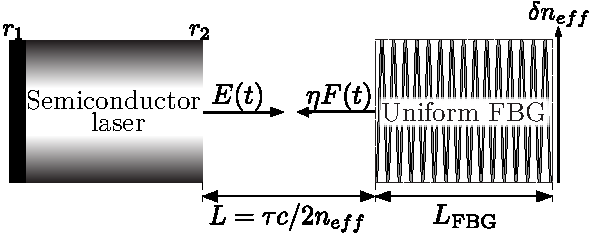
\includegraphics[width=\linewidth]{Images/FBG_setup_dneff_only_1col.pdf}

    \caption{Sketch of an optical fiber with an FBG written along its length.}

    \label{fig:FBG_setup}

\end{figure}
%
\par
%
It is defined as a repeating periodic variation $\delta n_{eff}(z)$ of the refractive index every $\Lambda$ along a length $L$ of a fiber. 
The number of gratings along an FBG is therefore $N = L/\Lambda$. The most general form for this periodic variation is given by
%
\begin{equation}
\label{eq:dneff}
    \delta n_{eff}(z) = \dnbar(z) \left[ 1 + v \cos{\left( \frac{2 \pi}{\Lambda} z + \phi(z) \right)} \right]
\end{equation}
%
where $\Lambda$ is the period of the grating, $\dnbar(z)$ is the profile of the periodic variations over $L$, for example, $\dnbar(z) \sim e^{-z^2}$ produces a Gaussian variation to the profile of the refractive index variation, 
$v$ is the fringe visibility of the index change, and $\phi(z)$ can vary the grating period along the fiber, allowing different frequencies to be reflected along the fiber's length.
%
\par
%
Light propagating through the fiber that interfaces with the FBG can undergo diffraction when its wavelength close to the design wavelength, given by $\lambda_D = 2 \neff \Lambda$. 
It is typically assumed that the light only undergoes first-order diffraction as this typically dominates in FBGs and thus a single propagating mode is considered. 
In this case, through the use of coupled-mode theory and the synchronous approximation, 
coupled first-order differential equations describing the interaction between the forward and backward propagating waves, $A(z)$ and $B(z)$, respectively, can be derived. 
See \cite{erdogan1997fiber} and references therein for further details.
%
\begin{equation}
\label{eq:wave_eqs}
    \begin{aligned}
        \frac{dR}{dz} &= i \hat{\sigma} R(z) + i \k S(z), \, R(z) = A(z) \exp{ \left( -i \left( \frac{\phi}{2} -\delta z \right) \right) }\\
        -\frac{dS}{dz} &= i \hat{\sigma} S(z) + i \k R(z), \, S(z) = B(z) \exp{ \left( -i \left( \frac{\phi}{2} + \delta z \right) \right) }
    \end{aligned}
\end{equation}
%
The terms $\delta$, referred to as the detuning, $\k$, referred to as the "AC" coupling coefficient and $\hat{\sigma}$, referred to as the general "dc" self-coupling coefficient, are given by
%
\begin{align}
    \label{eq:delta}
    \delta &= 2 \pi \neff \left( \frac{1}{\lambda} - \frac{1}{\lambda_D} \right) \\
    \label{eq:kappa}
    \k &= \frac{\pi}{\lambda} v \dnbar(z)\\
    \label{eq:sigma}
    \hat{\sigma} &= \frac{2\k}{v} + \delta -\frac{1}{2}\frac{d\phi}{dz}
\end{align}
%
As $\k$ and $\hat{\sigma}$ generally depend on $z$, \eqref{eq:wave_eqs} cannot usually be solved analytically, but they are easily solved numerically following the prescription of a particular $\Lambda$, $\neff$, $\dnbar(z)$, $\phi(z)$, and $L$. 
%
\par
%
At this point, we have all the necessary ingredients to calculate the key characteristic of an FBG - its reflectivity spectrum $\rho(\w)$. 
Physically speaking, one is most interested in the reflection spectrum of light being reflected at the front FBG interface with no reflection at the back FBG interface. 
Therefore, \eqref{eq:wave_eqs} is typically solved (by defining $z=0$ to be half way along the FBGs length) subject to the boundary conditions $R(-L/2)=1$ and $S(L/2)=0$ and integrating backwards from $L/2$ to $-L/2$, 
with the amplitude reflection coefficient then given by
%
\begin{equation}
\label{eq:rho}
    \rho = \frac{S(-L/2)}{R(-L/2)}
\end{equation}
%
Although closed-form expressions for $\rho(\w)$ are typically not possible, as \eqref{eq:wave_eqs} must be solved numerically, 
some commonly used gratings allow for analytic expressions for $\rho(\w)$ and thus give excellent insights into common properties of FBG reflection spectra.
%
%
\subsection{Uniform FBG reflection spectra $\rho_\text{Bragg}(\w)$}
\label{subsec:FBG_feedback}
%
The most basic FBG is called the uniform grating. 
Its grating chirp $\sfrac{d\phi}{dz} = 0$ and the apodization $\dnbar=\text{const.}$ so that its grating index variation given by $\eqref{eq:dneff}$ is essentially a sine wave as shown in Figure~\ref{fig:dneff}(a). 
Therefore, $\k, \, \hat{\sigma}$ are constant in $z$, allowing an analytic reflectivity spectrum $\rho(\w)$ to be calculated by solving \eqref{eq:wave_eqs} and subsequently evaluating \eqref{eq:rho}.
%
\begin{equation}
\label{eq:uniform_rho}
    \rho = \frac{-\k \sinh\left(\sqrt{\k^2 - \hat{\sigma}^2}L\right)}{\hat{\sigma} \sinh\left(\sqrt{\k^2 - \hat{\sigma}^2}L\right) + i\sqrt{\k^2 - \hat{\sigma}^2} \cosh\left(\sqrt{\k^2 - \hat{\sigma}^2}L\right)}
\end{equation}
%
Several interesting features of reflection spectra $\rho$ are most easily visualised by varying $\k L$ for a particular fixed $N$ against normalised frequency, given by \cite{erdogan1997fiber}
%
\begin{equation*}
    \frac{\omega}{\omega_\text{max}} = 1 + \frac{\hat{\sigma} L}{\pi N}
\end{equation*}
%
Figure~\ref{fig:uniform_spectra_varykL} illustrates representative amplitude reflectivity and phase curves for uniform gratings plotted against angular frequency, 
for gratings centred at the most commonly used laser wavelength of 1550 nm, with values of $\k L \in [0.5, 2, 5]$, and a fixed $N = 5000$. 
Increasing $N$ (and therefore increasing $L$) results in a narrower reflection bandwidth, while decreasing $N$ (and therefore decreasing $L$) leads to a broader one, assuming $\k L$ remains constant. 
Reflection spectra consist of a main lobe and a series of side lobes, partitioned by reflection zeros, spaced symmetrically (as a function of $\lambda$) on either side of it. 
For gratings with a low $\k L$ such as 0.5, the main lobe was a bandwidth, which we define as the interval between its reflection zeros, equal to twice that of its side lobes \cite{erdogan1997fiber}. 
Evidently, increasing $\k L$ not only increases the grating's maximum reflectivity, but additionally broadens the bandwidth of the main lobe while narrowing the bandwidth of the side lobes. 
Additionally, the phase variations are approximately linear for low reflectivities while becoming more distorted as $\k L$ increases.
%
\begin{figure}
    
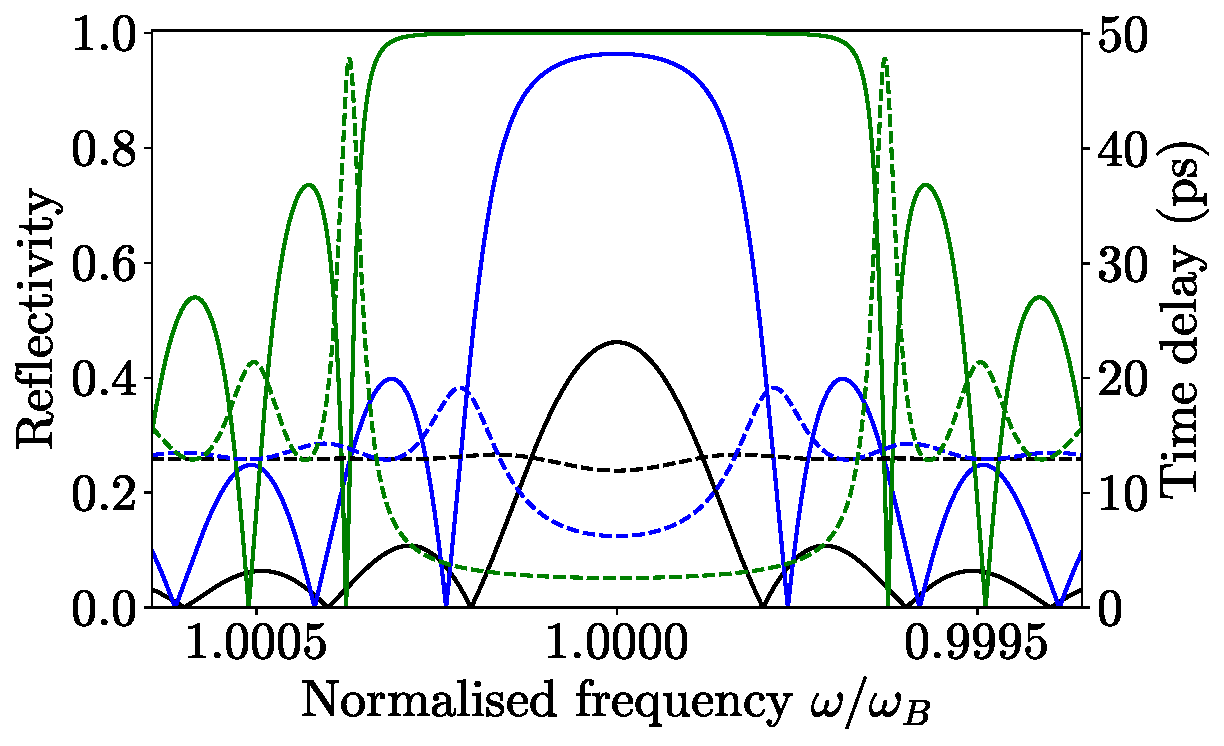
\includegraphics[width=\linewidth]{Images/Uniform_varying_kL_Rtau.pdf}

\caption{Examples of magnitude and phase of uniform FBG reflection spectra with varying dimensionless grating strength $\k L \in [0.5, 2, 5]$ and constant number of grating periods $N=5000$.}

\label{fig:uniform_spectra_varykL}
\end{figure}
%
\par
%
As $\k, \hat{\sigma}$ depend solely on $\lambda$ and the prescribed grating parameters, 
the reflected amplitude $|\rho|$ and reflected phase $\arg(\rho)$ can be immediately plotted against frequency by substituting \eqref{eq:kappa} and \eqref{eq:sigma} into \eqref{eq:uniform_rho}. 
Figure~\ref{fig:uniform_spectra_varyLdneff} shows some examples of the reflection spectra of uniform FBGs, now plotted against frequency, with their design frequency given by
%
\begin{equation}
    \w_D = \frac{\pi c}{\Lambda n_{eff}^2}
\end{equation}
%
highlighted to demonstrate the intrinsic detuning in the spectrum. The reflection spectrum of a uniform grating has a maximum reflectivity 
%
\begin{equation}
\label{eq:rmax}
    R \equiv |\rho_\text{max}| = \tanh{(\k L)}
\end{equation}
%
centred at the Bragg centre frequency $\w_c \equiv \omega_\text{max}$
%
\begin{equation}
\label{eq:wBragg}
    \w_c = \frac{\w_D}{\left( 1 + \frac{\dnbar }{\neff}\right)}
\end{equation}
%
We note that typically, $R$ is used for reflected power rather than reflected amplitude, but this choice of notation is made for clarity reasons in later sections. 
The phase at $\w_c$ is $\sfrac{\pi}{2}$ for all uniform gratings, while the reflection zeros are symmetric about $\w_c$, with the zeros either side of the main lobe occurring at $\w_c \pm \wz$, where
%
\begin{equation}
\label{eq:wz}
    \wz = \w_c \sqrt{\left( \frac{\dnbar}{2 \neff} \right)^2 + \frac{1}{N^2} }
\end{equation}
%
and the phase of the reflection spectrum varies by $2 \pi$ between the zeros. Outside of the main lobe, side lobe reflectivity peaks decay exponentially with periodic phase variations of $\pi$ within each lobe. 
Note the phase shift of $\pi$ between side lobes on either side of the reflectivity spectrum.
%
\par
%
Figure~\ref{fig:uniform_spectra_varyLdneff}(a) demonstrates the effect of doubling $L$ on reflection spectrum. 
Intuitively, $R$ increases for longer gratings as more gratings are available to prevent signal transmission. 
The bandwidth of each lobe decreases while the detuning from the design frequency is unchanged. When doubling $\dnbar$ as demonstrated in (b), $R$ is again increased. 
Conversely to (a), detuning increases while the grating bandwidth is unchanged. As these two parameters control the three features of the spectrum (detuning, maximum reflection, and bandwidth), 
one cannot vary a single feature of the reflection spectrum without additionally adjusting the grating period $\Lambda$, which can be used to compensate the detuning in $\w_c$ while having a negligible affect on $\wz$ and $R$. 
This is because optical lasers' centre frequencies are in THz while the amount of detuning is at most in GHz. Therefore, $\w_c/\w_D = \Lambda_D/\Lambda_c \approx 1$. 
Using this approximation, \eqref{eq:wBragg}, and \eqref{eq:wz}, $\dnbar, L, \Lambda$ can be calculated sequentially through the expressions
%
\begin{align}
\label{eq:spec2phys}
    \dnbar &\approx \frac{2\wz}{\w_c} \frac{\neff}{\sqrt{1 + \left(\frac{\pi}{\arctanh{(R)}} \right)^2}}
    \\
    \Lambda &= \frac{\pi c}{\w_c \neff (\neff +\dnbar)}
    \\
    L &= \frac{\Lambda}{\sqrt{\left( \frac{\wz}{\w_c} \right)^2 - \left( \frac{\dnbar}{2\neff} \right)^2}}
\end{align}
%
For example, if a uniform grating with a spectral response corresponding to $\w_c = 1.216\e{15}\; \text{rad s}^{-1}$, $\wz = 1\e{10}\; \text{rad s}^{-1}$, and $R = 0.5$ is desired, 
\eqref{eq:spec2phys} provides grating parameters $\dnbar= 4.2111838\e{-6}$, $\Lambda = 3.6494583\e{-7}\,\text{m}$, $L = 0.0444578955\,\text{m}$, 
which gives excellent agreement to the desired spectral response as shown in Figure~\ref{fig:spec2phys}.
%
%
\section*{FBG distributed feedback}
\label{sec:FBG_feedback}
%
Given the significant spectral advantages of FBGs for FOF and the straight-forward integration of FBGs into fiber optic semiconductor laser systems, 
investigations into their influence on the dynamics of external feedback semiconductor laser systems is of great interest. 
A sketch of the laser system under external feedback from an FBG is shown in Figure~\ref{fig:FBGF}. 
As demonstrated in the previous section, the reflectivity spectrum of FBGs can be rather complex. 
As an FBG in essence acts as a filter, the term $F(t)$ will be given by \eqref{eq:FOF} with $\rho(\w) = \rho_\text{Bragg}(\w)$. 
This term can alternatively be written as a convolution in the time domain,
%
\begin{equation}
    \label{eq:convolution}
     F(t) = e^{-i C_p} \tilde{\rho}_\text{Bragg}(t) \otimes E(t-\tau)
\end{equation}
%
where $\tilde{\rho}_\text{Bragg}(t)$ is the impulse response of the FBG with respect to the Bragg resonance frequency. 
Analytic expressions do not exist for the impulse response, even for simple gratings, and must therefore be calculated numerically through fast Fourier transforms (FFTs), for example. 
The requirement of numerically calculating $F(t)$ limits the analysis to numerical integration of solutions for $(E(t),N(t))$, and calculating properties of resulting time series, 
such as maximal Lyapunov exponents (MLEs) or spectral characteristics such as signal dispersion. 
Despite the obvious computational and analytical difficulties associated with this feedback term, 
research has been conducted into uniform FBG feedback using the convolution representation for $F(t)$ \cite{li2012distributed, li2015chaotic, li2020stable, jiang2021characterizing, skenderas2021feedback, skenderas2024impact}. 
In several studies, an expression for $\rho(\w)$ separates the reflection spectrum and detuning, allowing the detuning to be varied continuously while keeping the reflectivity spectrum shape constant. 
In this case, the reflected signal has the form,
%
\begin{equation*}
    F(t) = \eta e^{-i C_p} [\tilde{\rho}_0(t) e^{i \wB t}] \otimes E(t-\tau)
\end{equation*}
%
where $\tilde{\rho}_0$ is centred at the laser free-running frequency, while the detuning $\wB$ is an independent parameter. 
Although this form for the reflectivity distribution allows one to vary a single feature of the reflectivity distribution, as discussed in \ref{subsec:FBG_feedback}, the detuning and distribution shape intrinsically depend on each other, 
meaning that all grating parameters $\dnbar, \Lambda, L$ must be simultaneously adjusted in order to continuously detune over a constant distribution shape \cite{skenderas2024impact}. 
These parameters can be calculated for example through \eqref{eq:spec2phys}. 
Similarly, the distribution width and maximum reflectivity (occurring at $\w_c$) can only be independently varied through simultaneously varying all grating parameters.
%
\par
%
As numerical investigations only allow limited insights into the underlying dynamics of FBG feedback, initial numerical investigations focused on the potential of FBG feedback to produce high-quality chaotic signals. 
This is of research interest as chaotic signals produced by lasers subject to external feedback are used in a number of applications such as high-speed optical random bit generation \cite{uchida2008fast} and chaos-based secure communication \cite{annovazzi2008secure}. 
It was demonstrated that FBG feedback is more effective than conventional mirror feedback in suppressing the time-delay signature (TDS) associated with chaos generation in semiconductor lasers. 
TDS can limit the encryption capabilities of chaotic signals generated lasers subject to external feedback, as powerful autocorrelation algorithms can use a signal's TDS to partially or fully decrypt the signal \cite{rontani2007loss}. 
The improvement in TDS suppression was generally attributed to the time-distributed reflections provided by the FBG, `spreading out' the effective time delay of the chaotic signal \cite{li2012distributed}. 
Further, it was observed that TDS suppression improves as the bandwidth of the FBG decreases. This is linked to the increase in dispersion of the reflection group delay, which plays a crucial role in the dynamics of the laser. 
Notably, the length of the FBG does not significantly affect this suppression. 
Although narrower FBG bandwidth enhances chaotic signal TDS suppression, the size of parameter regions that exhibit chaos decrease, being replaced by regions of stable period-1 periodic orbits, 
in agreement with analyses of FOF \cite{li2020stable}, although it was demonstrated that in some cases, 
chaos can be induced by FBG feedback for lower time delays than what is possible using COF. 
Further investigations showed that optimal TDS suppression is achieved when the FBG is positively detuned from the laser frequency. 
The preference for positive detuning is attributed to the red-shifting of the laser cavity due to the anti-guidance effect \cite{li2015chaotic}. 
%
%From a dynamical systems perspective, these initial numerical investigations raised interesting questions on why there is an intrinsic asymmetry about the FBG spectrum in laser stability for positive or negative detuning and whether the laser frequency 
%
\par
%
The convolution representation for $F(t)$ under FBG feedback can alternatively be written as a distributed delay term. Using the definition of the convolution,
%
\begin{align*}
    \tilde{\rho}(t) \otimes E(t-\tau)
    &= \int_{-\infty}^{\infty} \tilde{\rho}(t-s) E(s-\tau) ds \\
    &= \int_{-\infty}^{t+\tau} \tilde{\rho}(t-s) E(s-\tau) ds
\end{align*}
%
as $E(s-\tau)=0$ for $s>t+\tau$. Now, choosing the lower bound $t-T$ so that $\tilde{\rho}(s) \approx 0 \; \forall \; s>T$.
%
\begin{equation*}
    \tilde{\rho}(t) \otimes E(t-\tau) \approx \int_{t-T}^{t+\tau} \tilde{\rho}(t-s) E(s - \tau) ds
\end{equation*}
%
This equivalent expression for $F(t)$ has been used in further numerical studies on the use of chirped FBGs (CFBGs), 
which are of interest in TDS suppression due to their enhanced dispersion characteristics compared to the previously explored uniform FBGs \cite{wang2017time, wang2019key, wang2023critical, chao2020permutation}. 
An illustration of the index profile of CFBGs is given in Figure~\ref{fig:dneff}(d). 
As there are no analytic expressions for a chirped reflectivity spectrum compared to a uniform one, \eqref{eq:wave_eqs} must be solved numerically, further increasing computational complexity. 
The impulse response $\tilde{\rho}(t)$ involved in the distributed feedback is calculated through FFTs as done in previous investigations. 
Investigations into CFBG feedback demonstrated enhanced TDS compared to uniform FBG feedback, eliminating TDS without requiring amplification, simplifying system configuration.
%
\par
%
More recently, investigations have gone beyond studying chaotic signal generation but similar to the previous analyses, the convolution representation for $F(t)$, restricted computations to basic time series generation. 
\Skenderas \textit{et al.} observed that the location of the zeros of the reflectivity spectrum, can strongly influence laser stability. 
They demonstrated that these stability fluctuations are likely due the damping of relaxation oscillations (ROs) when the zeros of the FBG reflectivity spectrum is aligned with the laser's RO frequency ($\w_{RO}$) side lobes. 
These stability fluctuations were found by tracking the required feedback rate to produce a Hopf bifurcation, that is, where constant intensity emission begins to periodically fluctuate, for increasing the FBG length which in turn decreases FBG bandwidth. 
As changing FBG length changes its reflectivity, the other FBG parameters are required to be adjusted to ensure a constant reflectivity. 
Asymmetry in stability fluctuations were observed for frequency detuning relative to the Bragg wavelength, as was the case in previous studies \cite{li2012distributed}, but alternatively attributed to the frequency-dependent phase shift induced by the FBG \cite{skenderas2024impact, skenderas2021feedback}. 
This gives further indication that the observed asymmetrical behaviour with respect to detuning emerges as an intrinsic characteristic of FBG feedback. Overall, the numerical simulations reveal that FBG feedback shares many features with FOF. 
However, the precise shape, location of reflection zeros, and, most notably, the phase of the FBG introduce additional complexity. 
%
\par
%
While the representation of $F(t)$ as a convolution has been shown to provide some limited insights into FBG feedback, an alternative form for $F(t)$ has been shown to allow deeper analyses into its associated dynamics. 
The case of FBG feedback subject to strong feedback was considered in a series of papers by Naumenko \textit{et al.} \cite{naumenko2003characteristics, naumenko2004slow, besnard2002intensity}. 
The modified rate equations used in the analysis are based on a model first proposed in 1989 \cite{rong1989improved} describing strong feedback due to a plain mirror. 
They replace the feedback term $\eta e^{-i C_p} E(t-\tau)$ in the LK rate equations with the term $E(t) \ln{\left[ E_r(t) / E(t) \right]}$ where $E_r(t)$ accounts for the multiple EC reflections caused by the strong COF, 
similar to \eqref{eq:multiple_EC} by defining
%
\begin{equation*}
    E_r(t) = E(t) + \frac{R_2^2 - 1}{R_2^2} \sum_{n=1}^\infty (-R_2 R)^n e^{-i n C_p} E(t-n \tau)
\end{equation*}
%
Indeed, truncating this expression for $F(t)$ to first order reduces to single reflection feedback. Taking the Taylor expansion of the logarithm,
%
\begin{equation*}
    \begin{aligned}
        &E(t) \ln{\left[ \frac{E_r(t)}{E(t)} \right]} = \sum_{n=1}^\infty \frac{(-1)^{n-1}}{n}\left( \frac{E_r(t)}{E(t)} - 1\right)^n \\
        &\,\overset{n=1}{\approx} E(t)\left( \frac{E(t) + \frac{R_2^2 - 1}{R_2^2}(-R_2 R)e^{-i C_p} E(t - \tau) - E(t)}{E(t)} \right)\\
        &\;\;= \eta e^{-i C_p} E(t - \tau)
    \end{aligned}   
\end{equation*}
%
as desired.
Reflection due to an FBG can be modelled by modifying this expression to account for the spectral filtering $\rho_{\text{Bragg}}(\w)$ of the grating. 
Multiple reflections given by the terms $(R_2 R)^n e^{-i n C_p} E(t-n \tau)$ are now replaced by terms given by \eqref{eq:FOF}, see Appendix~\ref{sec:multiple_EC_nondim} for details. 
Through the use of Green's functions, an expression for the ECMs of the system can be derived, allowing for significantly deeper insights into the dynamics compared to the convolution method discussed previously. 
It was shown that under weak feedback, the stationary ECM states are mostly confined to the main lobe of the gratings reflectivity spectrum, while the MGM is shifted close to $\wB=0$, 
identical to the results presented by Yousefi and Lenstra in the case of FOF. 
They additionally identified `satellite' ECMs, for narrow bandwidth FBGs, separated from the central ECM ellipse by the zeros of the main lobe. 
It is shown that under strong feedback conditions that narrow filters lead to the excitation of additional solutions confined to the side lobes of the FBG frequency response. 
Although numerical integration of the presented system can be performed, and stationary states calculated, 
the complexity of $F(t)$ prevents the use of advanced bifurcation tools such as numerical continuation and stability analysis of the stationary solutions, clouding the underlying dynamics induced by the frequency-dependent FBG reflection. 
%
\par
%
The similarities in the results of Naumenko \textit{et al.} to work on FOF is fairly evident when one considers a single reflection. 
Carrying out the same first-order approximation on this feedback term yields an equivalent feedback term as used in the original FOF definition considered by Yousefi and Lenstra with $\rho(\w) = \rho_\text{Bragg}(\w)$. 
See Appendix~\ref{sec:multiple_EC_nondim} for further details. 
Therefore, it is natural to ask if there is a an approximation to $\rho_\text{Bragg}(w)$ which captures its key frequency-dependent reflection effects while enabling the feedback term $\eta F(t)$ to be reduced to DDEs which amenable to advanced bifurcation analysis.